\section{Vorgehensmodelle}
\begin{frame}[fragile]
\frametitle{Vorgehensmodelle}
\huge Vorgehensmodelle
\end{frame}

\begin{frame}
\frametitle{Begriffe}
	\begin{block}{Definition ``Prozess'' nach IEEE}
		Eine Folge von Schritten die zu einem definierten Zweck ausgeführt werden
		\begin{itemize}
			\item Beispielsweise der Softwareentwicklungsprozess
			\item Um Operationen auf Daten auszuführen
		\end{itemize}
		von Software.
	\end{block}	
\end{frame}

\begin{frame}
\frametitle{Begriffe}
	\begin{block}{Definition ``Softwareentwicklungsprozess'' nach IEEE}
		Der Prozess bei dem die Bedürfnisse von Nutzern in ein Softwareprodukt übersetzt werden.
		Der Prozess beeinhaltet
		\begin{itemize}
			\item das Übersetzen der Bedürfnisse in konkrete Anforderungen,
			\item die Überführen der Anforderungen in einen Entwurf,
			\item die Implementierung des Entwurfs in Quelltext,
			\item das Testen des Quelltextes,
			\item die Installation und den Betrieg der implementierten Software.
		\end{itemize}
	\end{block}	
\end{frame}

\begin{frame}
\frametitle{Softwareentwicklungsprozesse in der Praxis}
\begin{itemize}
	\item Softwareprozesse variieren je nach Organisation
	\item kein Prozess ist perfekt
	\item Folge: Ergebnisse unterscheiden sich situationsbedingt
\end{itemize}
\end{frame}

\begin{frame}
\frametitle{Übung 2.1}
	Geben Sie
	\begin{enumerate}
		\item Beispiele für unterschiedliche Softwareprozesse
		\item Gründe für diese Unterschiede
	\end{enumerate}
	Warum ist es schwierig Softwareentwicklungsprozesse zu automatisieren?
\end{frame}

\ifloesung
\begin{frame}
\frametitle{Übung 2.1 - Lösung}
	\scriptsize
	Beispiele für unterschiedliche Softwareprozesse
	\begin{enumerate}
		\item Planungsgetriebene Prozesse
		\begin{itemize}
			\item Sequenziell
			\item Nebenläufig
			\item Inkrementell
		\end{itemize}
		\item Agile Prozesse
		\item \ldots
	\end{enumerate}
	\bigskip
	Gründe für diese Unterschiede
	\begin{enumerate}
		\item Detailgrad der Anforderungen
		\item Teamstruktur
		\item Planbarkeit des Softwareprodukts
		\item Time-2-Market
		\item Art der Software die Entwickelt wird
		\item Kundentyp
		\item \ldots
	\end{enumerate}
	\normalsize
\end{frame}

\begin{frame}
\frametitle{Übung 2.1 - Lösung}
	\scriptsize
	Warum ist es schwierig Softwareentwicklungsprozesse zu automatisieren?
	\begin{enumerate}
		\item Anforderungen oft nicht final
		\item Komplexe Systeme sehr schwer zu testen
		\item Große Systeme besitzen viele Schnittstellen
		\item \ldots
	\end{enumerate}
	\normalsize
\end{frame}
\fi

\begin{frame}
\frametitle{Prozessmodell vs konkreter Prozess}
	Modell
		\begin{itemize}
			\item Abstrakte Abfolge von Schritten
			\item Dient beliebig vielen Prozessen als Grundlage für konkretes Vorgehen
			\item Ist ein Muster für eine bestimmte Vorgehensweise
		\end{itemize}
	\bigskip
	Prozess = Gegenstand des Modells
		\begin{itemize}
			\item Tatsächlich ausgeführte Abfolge von Schritten
			\item Jeder Schritt produziert konkretes Ergebniss
			\item Ist das Projekt
		\end{itemize}
\end{frame}

\begin{frame}
\frametitle{Beispiele Modell vs konkreter Gegenstand}
	\begin{columns}
		\begin{column}{0.5\textwidth}
		Modell
			\small
			\begin{itemize}
				\item Theaterstück
				\item Musik-CD
				\item Applikation
				\item Klasse
				\item Vorgehensmodell
				\item Prozessmodell
			\end{itemize}
			\normalsize
		\end{column}
		\begin{column}{.5\textwidth}
		Gegenstand
			\small
			\begin{itemize}
				\item Aufführung
				\item Einmalige Wiedergabe
				\item Ausführung der Applikation
				\item Objekt
				\item Projektablauf
				\item Projekt (inkl. Organisation)
			\end{itemize}
			\normalsize
		\end{column}
	\end{columns}
\end{frame}

\begin{frame}
\frametitle{Merkmale von Modellen}
	Abbildungsmerkmal
	\begin{itemize}
		\item Ein Modell ist immer ein Abbild des Originals
		\item dass 
		\begin{itemize}
			\item Struktur (z.B. Aufbau eines Hauses), 
			\item Verhalten (z.B. Schiffsmodell im Strömungskanal)
			\item oder Funktionsweise (z.B. Modellauto dass fährt)
		\end{itemize}
		des Originals abbildet.
	\end{itemize}
	\bigskip
	Verkürzungsmerkmal
	\begin{itemize}
		\item Es enthält die relevanten Eigenschaften wie
		\begin{itemize}
			\item detaillierter Skelettaufbau des Menschen für Ärzte
			\item oder die Beschreibung der Proportionen des Menschen für Schneider
		\end{itemize}
	\end{itemize}
	\bigskip
	Pragmatisches Merkmal
	\begin{itemize}
		\item Es ist zugeschnitten auf den Untersuchungszweck und kann damit
		unter bestimmten Bedingungen das Original ersetzen
	\end{itemize}
	\bigskip
\end{frame}

\begin{frame}
\frametitle{Modelle beim Software Engineering}
	Software wird auf unterschiedliche Arten repräsentiert (Software Modelle)
		\begin{itemize}
			\item Spezifikation
			\item Entwurf
			\item Diagramme
			\item Code
			\item Kennzahlen
			\item Dokumentation
		\end{itemize}
	\bigskip
	Abläufe bei der Entwicklung von Software werden durch Vorgehens-/Prozessmodelle beschrieben
\end{frame}

\subsection{Basismodelle}
\begin{frame}
\frametitle{Basismodelle}
\huge Basismodelle
\end{frame}

\begin{frame}
\frametitle{Basismodelle}
	\begin{block}{Definition Vorgehensmodell}
		Darstellung, die weitgehend den Softwareentwicklungsprozess beschreibt und prinzipiell 
		auch Analysen des Prozesses gestattet.
		Ein Vorgehensmodell muss die Prozessschritte und die dabei verwendeten und entwickelten 
		Resultate explizit beschreiben.
	\end{block}
\end{frame}

\begin{frame}
\frametitle{Code and Fix}
	
\end{frame}

\begin{frame}
\frametitle{Sequenzielles Modell}
	
\end{frame}

\begin{frame}
\frametitle{Wasserfallmodell als bekanntestes sequentielles Modell}
	
\end{frame}

\begin{frame}
\frametitle{Nebenläufiges Modell}
	
\end{frame}

\begin{frame}
\frametitle{Inkrementelles Modell}
	
\end{frame}

\begin{frame}
\frametitle{Evolutionäres Modell}
	
\end{frame}

\begin{frame}
\frametitle{Prototypen}
	
\end{frame}

\begin{frame}
\frametitle{Pilotsystem}
	
\end{frame}

\begin{frame}
\frametitle{Spiralmodell}
	
\end{frame}

\subsection{Monumentale Prozessmodelle}
\begin{frame}
\frametitle{Monumentale Prozessmodelle}
\huge Monumentale Prozessmodelle
\end{frame}

\begin{frame}
\frametitle{Monumentale Prozessmodelle}
	\begin{block}{Definition Prozessmodell}
		Während Vorgehensmodelle den Kern bilden, ergänzen Prozessmodelle die Vorgehensmodelle um 
		Organisationsstrukturen für Projektmanagement, Qualitätssicherung, Dokumentation sowie 
		Konfigurationsverwaltung.
	\end{block}
\end{frame}

\begin{frame}
\frametitle{Monumentale Prozessmodelle}
	\begin{itemize}
		\item Aktivitäten werden von Mitarbeitern durchgeführt
		\item Die Kenntnisse/Fähgikeiten die als Vorraussetzung dienen
		werden durch Rollen beschrieben
		\item Die Durchführung wird genauer spezifiziert
		\begin{itemize}
			\item Weitere durchzuführende Aktivität?
			\item Rollenzuordnung
			\item Zu verwendende Artifakte
			\item Zu erstellende Artifakte
			\item Zu beachtende Konventionen, Methoden, Richtlinien
			\item Einzusetzende Werkzeuge
		\end{itemize}
	\end{itemize}
\end{frame}

\begin{frame}
\frametitle{Monumentale Prozessmodelle}
	\center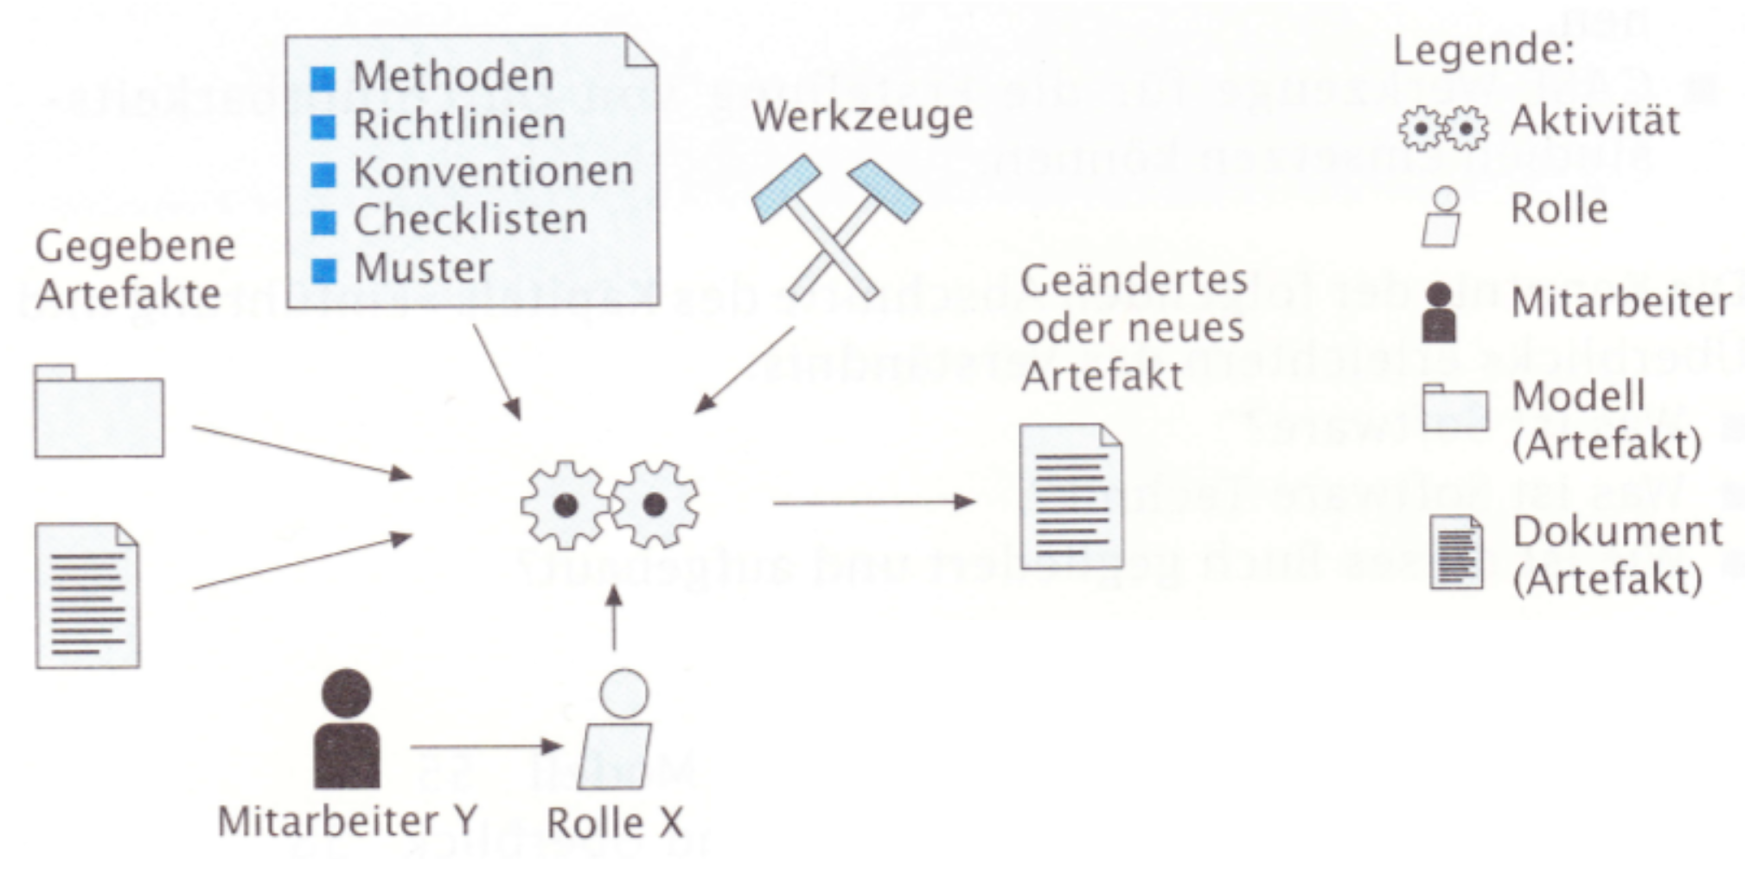
\includegraphics[width=1\textwidth,
			keepaspectratio=true]{bilder/prozessmodell.png}
\end{frame}

\begin{frame}
\frametitle{V-Modell}
	
\end{frame}

\begin{frame}
\frametitle{Rational Unified Process}
	
\end{frame}

\subsection{Agile Prozessmodelle}
\begin{frame}
\frametitle{Agile Prozessmodelle}
\huge Agile Prozessmodelle
\end{frame}

\begin{frame}
\frametitle{Agile Prozessmodelle}

\end{frame}

\begin{frame}
\frametitle{Extreme Programming}
	
\end{frame}

\begin{frame}
\frametitle{Scrum}
	
\end{frame}

\begin{frame}
\frametitle{Kanban}
	
\end{frame}
